%!TEX encoding = IsoLatin

%% Document is article 
\documentclass[a4paper]{article}

%% ----------------------------------------------------- PACKAGES ----------------------------------------------------- %%
\usepackage{coolArticle}
\usepackage[ruled]{algorithm2e}


%% ---------------------------------------------------- DOCUMENT ---------------------------------------------------- %%
\begin{document}

\noindent \textsc{Gallois-Montbrun} Gr�goire\\
\textsc{Faury} Louis 
	\titlebox{0.6}{Model Predictive Control}{Exercise \#3 - \textcolor{blue}{Group 2}}
	
	\section{Ex.1 : Computing invariant sets}
	{
		\paragraph{} We consider the following discrete time linear time-invariant system : 
		\begin{equation}
			x^+ = Ax 
			\label{system}
		\end{equation}
		with : 
		\begin{equation}
			A = \begin{bmatrix} \cos{(\alpha)} & \sin{(\alpha)} \\ -\sin{(\alpha)} & cos{(\alpha)} \end{bmatrix} \beta
			\label{matrixA}
		\end{equation}
		and $\beta = 0.6$ and $\alpha = \frac{\pi}{6}$. 
		We also introduce the constraint set :
		\begin{equation}
			\mathbb{X} = \left\{ x\, \vert \, Hx \leq h\right\} \quad \text{ where } H = \begin{bmatrix} \cos{(\pi/3)} & \sin{(\pi/3)} \\ -\cos{(\pi/3)} & -\sin{(\pi/3)} \\ \sin{(\pi/3)} & -\cos{(\pi/3)} \\ -\sin{(\pi/3)} & \cos{(\pi/3)} \end{bmatrix} \, \text{ and } h = \begin{bmatrix}  2 & 1 & 2 & 5 \end{bmatrix}^T
			\label{stateconstraints}
		\end{equation}

		\paragraph{} $\color{red}\blacktriangleright$ We are going to implement the following algorithm : 
		\vspace{10pt}	
			
		\begin{algorithm}[H]
			\SetKwRepeat{Do}{do}{while}
	 		\SetAlgoLined
			\KwData{$\mathbb{X}$, $A$} 
			\KwResult{$\mathcal{O}_{\infty}$} 
			1.  Initialize : $\Omega_0 = \mathbb{X}$ \\
			2. \Do{$\Omega_{i+1}=\Omega_i$}
			{
				$\Omega_{i+1} = pre(\Omega_i)\cap \Omega_i $
			}
			3. $\mathcal{O}_{\infty} = \Omega_i$
			\caption{Maximum invariant set computation}
		\end{algorithm}
		\vspace{10pt}
		
		\noindent in order to compute the maximum invariant set contained in $\mathbb{X}$. The computations are made tractable by the linearity of our transition model as well as by the polytopal description of our different sets. The Matlab code performing this operations is provided with this report. 
		
		\begin{figure}[h!]
			\begin{minipage}{0.5\linewidth}
			{
				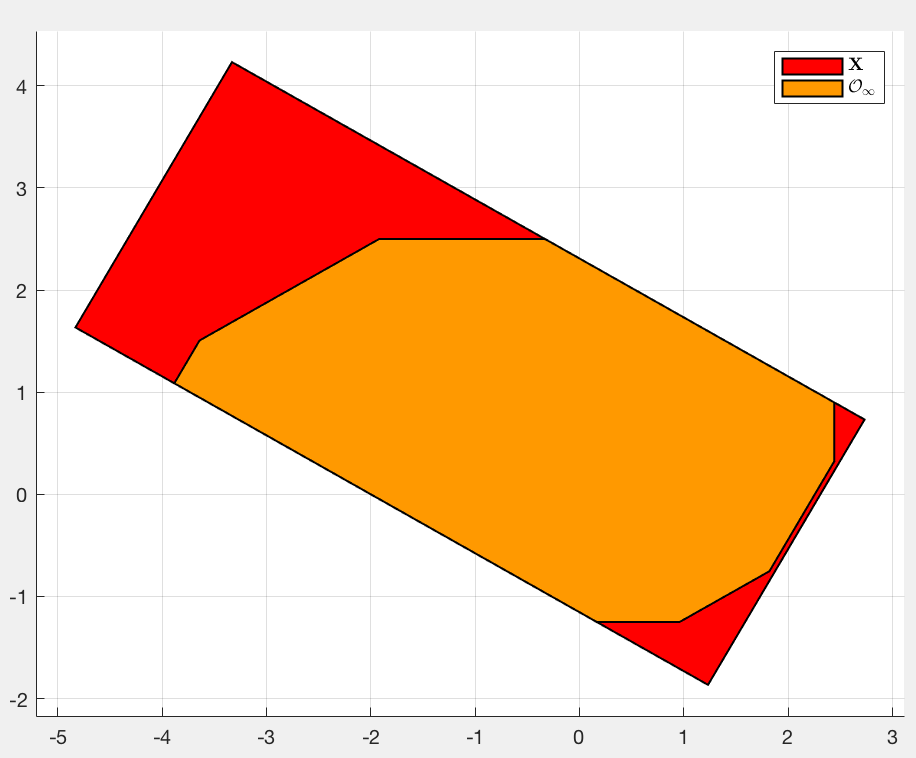
\includegraphics[width=0.95\linewidth]{feasible_set}
				\label{fig::max_inv}
				\caption{Feasible and maximum invariant set}
			}
			\end{minipage}
			\begin{minipage}{0.5\linewidth}
			{
				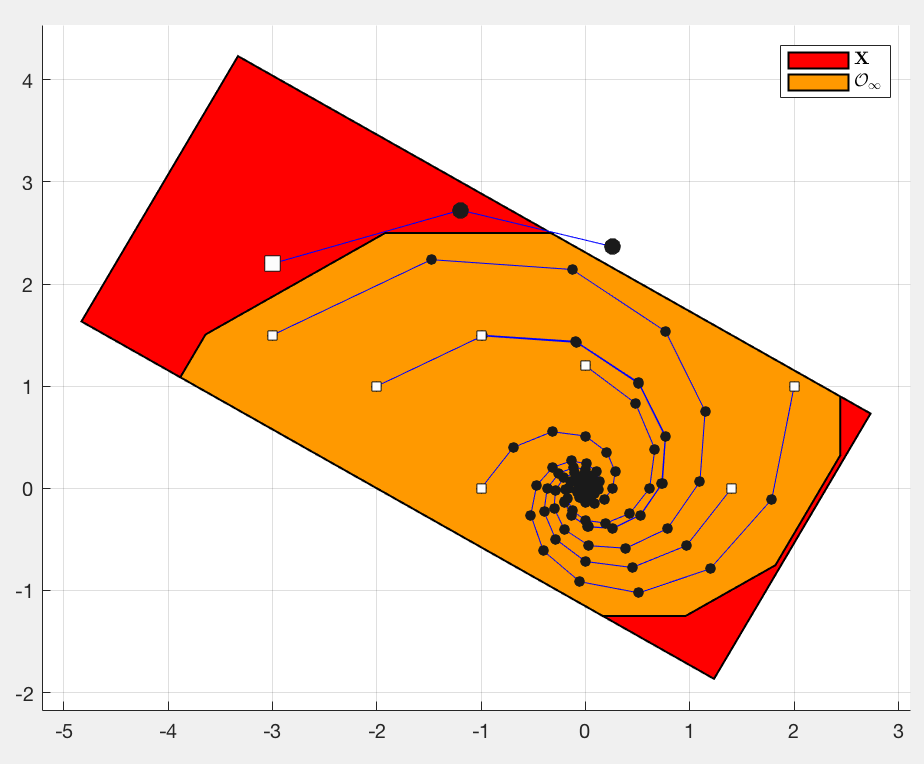
\includegraphics[width=0.95\linewidth]{feasible_traj}
				\label{fig::traj}
				\caption{Trajectories plot}
			}
			\end{minipage}
		\end{figure}
		
		\paragraph{} $\color{red}\blacktriangleright$ Figure (\ref{fig::max_inv}) displays the maximum invariant set as well as the feasible set. Figure (\ref{fig::traj}) plots 6 different trajectories starting in $\mathcal{O}_\infty$ as well as one trajectory starting in $\mathbb{X}\backslash\mathcal{O}_\infty$. One can notice that as expected, all trajectory starting in $\mathcal{O}_\infty$ remains in that set (and hence remain feasible) for all time, as they converge towards the origin. On the other hand, we notice that the only trajectory starting outside of the maximum invariant set quickly leaves the feasible set. 
	} 
		
	\section{Ex.2 : Computing controlled invariant sets}
	{
	\paragraph{} $\color{red}\blacktriangleright$ Here we intend to compute the maximum controlled invariant set of the system defined as :
		\begin{equation}
			x^+ = Ax + Bu
			\label{controlled}
		\end{equation}
		with :
		 \begin{equation}
			A = \begin{bmatrix} \cos{(\alpha)} & \sin{(\alpha)} \\ -\sin{(\alpha)} & cos{(\alpha)} \end{bmatrix} \beta \quad \alpha = \frac{\pi}{6} \quad \beta=0.6 \quad \text{and } B = \begin{pmatrix} 0.5\\ 0.5\end{pmatrix}
  		  \end{equation}
	The system is constrained such that $x\in\mathbb{X}$ and $u\in\mathbb{U}$ with : 
		\begin{equation}
			\mathbb{X} = \left\{ x\, \vert \, Hx \leq h\right\} \quad \text{and } \quad \mathbb{U} = \left\{ u\,\vert -0.5 \leq u \leq 0.5\right\}
			\label{inputconstraints}
		\end{equation}
		\vspace{10pt}	
		
		We therefore apply the following algorithm:\\
		\begin{algorithm}[H]
			\SetKwRepeat{Do}{do}{while}
	 		\SetAlgoLined
			\KwData{$\mathbb{X}$,  $\mathbb{U}$, $A$} 
			\KwResult{$\mathcal{C}_{\infty}$} 
			1.  Initialize : $\Omega_0 = \mathbb{X}$ \\
			2. \Do{$\Omega_{i+1}=\Omega_i$}
			{
				$\Omega_{i+1} = pre(\Omega_i)\cap \Omega_i $
			}
			3. $\mathcal{C}_{\infty} = \Omega_i$
			\caption{Maximum controlled invariant set computation}
		\end{algorithm}
		\vspace{10pt}
		
		where  for $\Omega\subset\mathbb{X}$, $pre(\Omega)$ consists in the following projection:
		\begin{equation}
			pre(\Omega) = \left\{x\in\mathbb{X}\,\vert\, \exists u\in\mathbb{U}, \begin{bmatrix}H_\Omega A & H_\Omega B \\
			0 &G\end{bmatrix} \begin{pmatrix} x \\ u\end{pmatrix}\leq \begin{bmatrix}b_\Omega \\ g\end{bmatrix}\right\} \quad \text{with $b_\Omega$  and $H_\Omega$ such that } \Omega =\left\{x\,\vert H_\Omega x\leq b_\Omega\right\}
		\end{equation}
		 and:
		\begin{equation}
		G = \begin{bmatrix}1 \\ -1\end{bmatrix}, \quad g =\begin{bmatrix}0.5 \\ 0.5\end{bmatrix}
		\end{equation}
		
		\begin{figure}[h!]
				\centering
				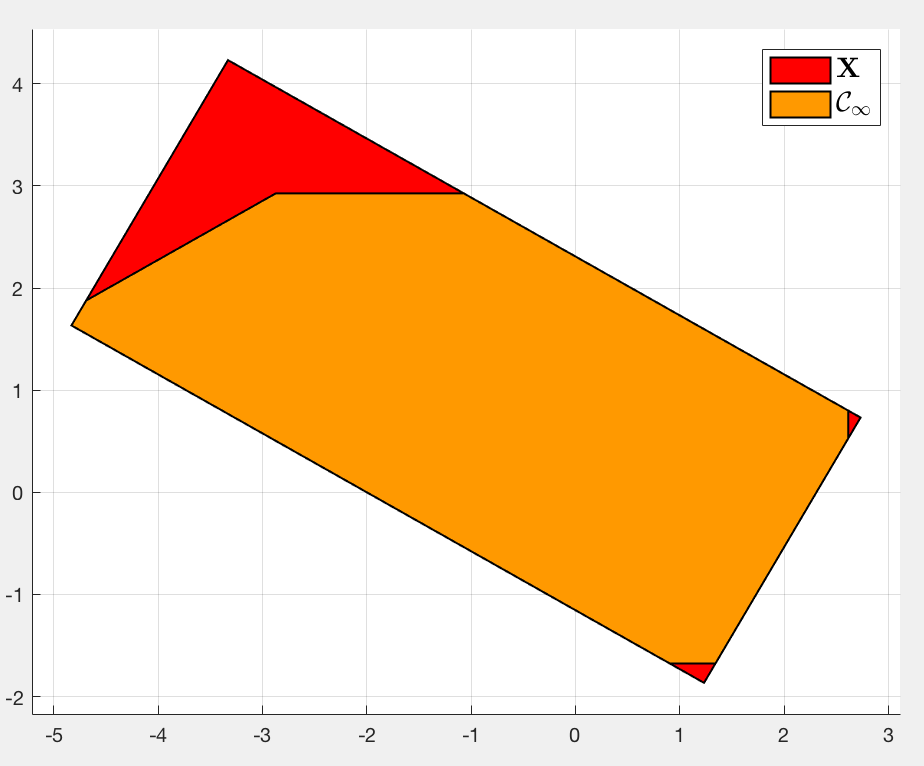
\includegraphics[scale=0.5]{ctrld_invariant_set}
				\label{fig::max_Ctrlinv}
				\caption{Feasible and maximum controlled invariant set}
		\end{figure}
		
		\paragraph{}
		Computed maximum controlled invariant is displayed on figure (\ref{fig::max_Ctrlinv}). We of course  have $\mathbb{C}_\infty\subset\mathbb{X}$. We also have $\mathbb{O}_\infty\subset\mathbb{C}_\infty$, all points in $\mathbb{O}_\infty$ indeed correspond to the particular case where $u=0$ ($\left\{0\right\}\subset\mathbb{U}$).
		
		
		\paragraph{} $\color{red}\blacktriangleright$ We now consider the system controlled by the optimal LQR control sequence $u^*$ corresponding to the following optimization problem:
		\begin{equation}
		\begin{split} 
				u^*= argmin\left\{ \sum\limits_{i=0}^\infty x_i^T Qx_i+u_i^TRu_i\right\} \\
		 		\text{s.t}\quad x_{i+1}=Ax_i+Bu_i
		\end{split}
		\end{equation}
		with :
		\begin{equation}
		Q = I \quad \text{and }R = 1.
		\end{equation}
		
		\paragraph{}
		The solution to this problem is defined as :
		\begin{equation}
		\forall i \quad u_i=Kx_i\quad \text{with } K=-(R+B^TPB)^{-1}B^TPA 
		\end{equation}
		where $P$ is the solution of the discrete-time algebraic Riccati equation:
		\begin{equation}
		P=Q+A^TPA-A^TPB(R+B^TPB)^{-1}B^TPA
		\end{equation}
		
		\paragraph{}
		The LQR controlled system is therefore defined as:
		\begin{equation}
		x^+ = (A+BK)x
		\end{equation}
		with constraint:
		\begin{equation}
		x\in\mathbb{X}\cap K\mathbb{U}=\mathbb{X}^{lqr}
		\end{equation}
		
		Its maximum invariant set $\mathcal{O}^{lqr}_\infty$ is then computed applying algorithm (1), following the same principle as in the previous exercise. Figure (\ref{fig::invariant_lqr}) shows the different sets computed so far. We notice that $\mathcal{O}_\infty^{lqr}\subset\mathcal{C}_\infty$ due to the fact that the new defined LQR controlled system corresponds to a particular case of the system defined as equation (\ref{controlled}). $\mathcal{O}_\infty^{lqr}$ is therefore smaller than $\mathcal{C}_\infty$
		
		
		\begin{figure}[h!]
				\centering
				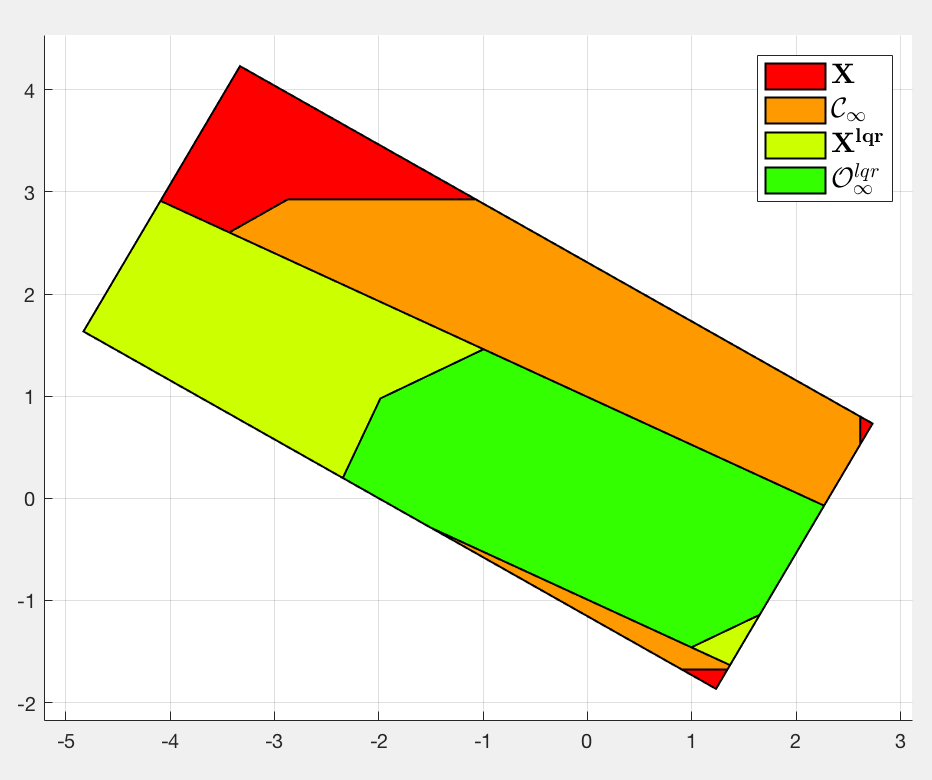
\includegraphics[scale=0.5]{lqr_sets}
				\label{fig::invariant_lqr}
				\caption{$\mathbb{X}$,  $\mathbb{X}^{lqr}$, $\mathcal{C}^\infty$ and $\mathcal{O}_\infty^{lqr}$}
		\end{figure}
		
	}
	
	\section{Ex.3 : Q\&A}
	{
		\paragraph{} We hereinafter consider the system : 
		\begin{equation}
			x^+ = f(x,u) \quad (x,u)\in\mathbb{X}\times\mathbb{U}
		\end{equation}
		
		\begin{enumerate}
			\item If $A$ is the maximum invariant set for 
			\begin{equation}
				x^+ = f(x,\mu(x)) 
			\end{equation}
			therefore $A\subseteq B$ where $B$ is the maximum control invariant set for $f(x,u)$. Indeed, $A$ correspond to a particular case of $B$ where we consider a feedback controller, whereas in $B$ all kinds of control laws can be considered. Therefore : 
			\begin{equation}
				\forall x \in A, \, \mathcal{X}(x,t) \in B \text{ for all } t>0
			\end{equation}
			where $\mathcal{X}(x,t)$ denotes the flow of the solution starting at $x$ for $t=0$. Therefore 
			\begin{equation}
				\color{red}
				A \subseteq B
			\end{equation}
			
			\item  Let $\mathcal{C}$ be a control invariant set for the system and $x\in\mathcal{C}$. The definition of a controlled invariant set ensures that there exits a control law such that the state $x$ will always stay in $\mathcal{C}$. However, nothing ensures that this holds for all controls and therefore \color{red}in the general case there can exist a control $u$ such that $f(x, u)\notin\mathcal{C}$.
		\end{enumerate}
		
		

	}
	
	
	
	
	
\end{document}